\header{
    \section{La Piémontaise} \label{la-piemontaise}
    %
    \insertComment{Chanson de \~1705 racontant la conquête puis la perte du Piémont par Henri IV.}{}
}

\enluminure{2}{\href{https://www.youtube.com/watch?v=KuHmFeAqmbg}{G}}{rands} dieux ! Que je suis à mon aise
\\Quand j’ai ma mie auprès de moi, auprès de moi !
\\
\bisdoublespace{De temps en temps, je la regarde}
{Et je lui dit : embrasse moi, embrasse moi !}
\\\\Comment veux-tu que je t’embrasse
\\Quand on me dit du mal de toi, du mal de toi ?
\\
\bisdoublespace{On dit que tu pars pour la guerre}
{Dans le Piémont servir le roi, servir le roi.}
\\\\Ceux qui t’ont dit cela, ma belle,
\\Ils t’ont bien dit la vérité, la vérité.
\\
\bisdoublespace{Mon cheval est à l’écurie,}
{Sellé, bridé, prêt à partir, prêt à partir !}
\\\\Quand tu seras dans ces campagnes,
\\Tu n’y penseras plus à moi, non plus à moi.
\\
\bisdoublespace{Tu n’penseras qu’aux Piémontaises}
{Qui sont cent fois plus belles que moi, plus belles que moi.}
\\\\Si fait, si fait, si fait, ma belle,
\\J’y penserai toujours à toi, toujours à toi.
\\
\bisdoublespace{Je ferai faire une belle image}
{Toute à la semblance de toi, semblance de toi.}
\\\\Quand je serai z’a table à boire,
\\A mes camarades je dirai, oui je dirai :
\\
\bisdoublespace{Chers camarades, venez voir,}
{Celle que mon cœur a tant aimée, a tant aimée !}
\\\\Je l’ai aimée, je l’aime encore,
\\Je l’aimerai tant que je vivrai, que je vivrai.
\\
\bisdoublespace{Je l’aimerai quand je serai mort}
{Si c’est donné aux trépassés, aux trépassés.}
\\\\Alors, j'ai tant versé de larmes
\\Que trois moulins en ont tourné, en ont tourné.
\\
\bisdoublespace{Petits ruisseaux, grandes rivières}
{Pendant trois jours ont débordé, ont débordé!}
\bigskip
\begin{center}
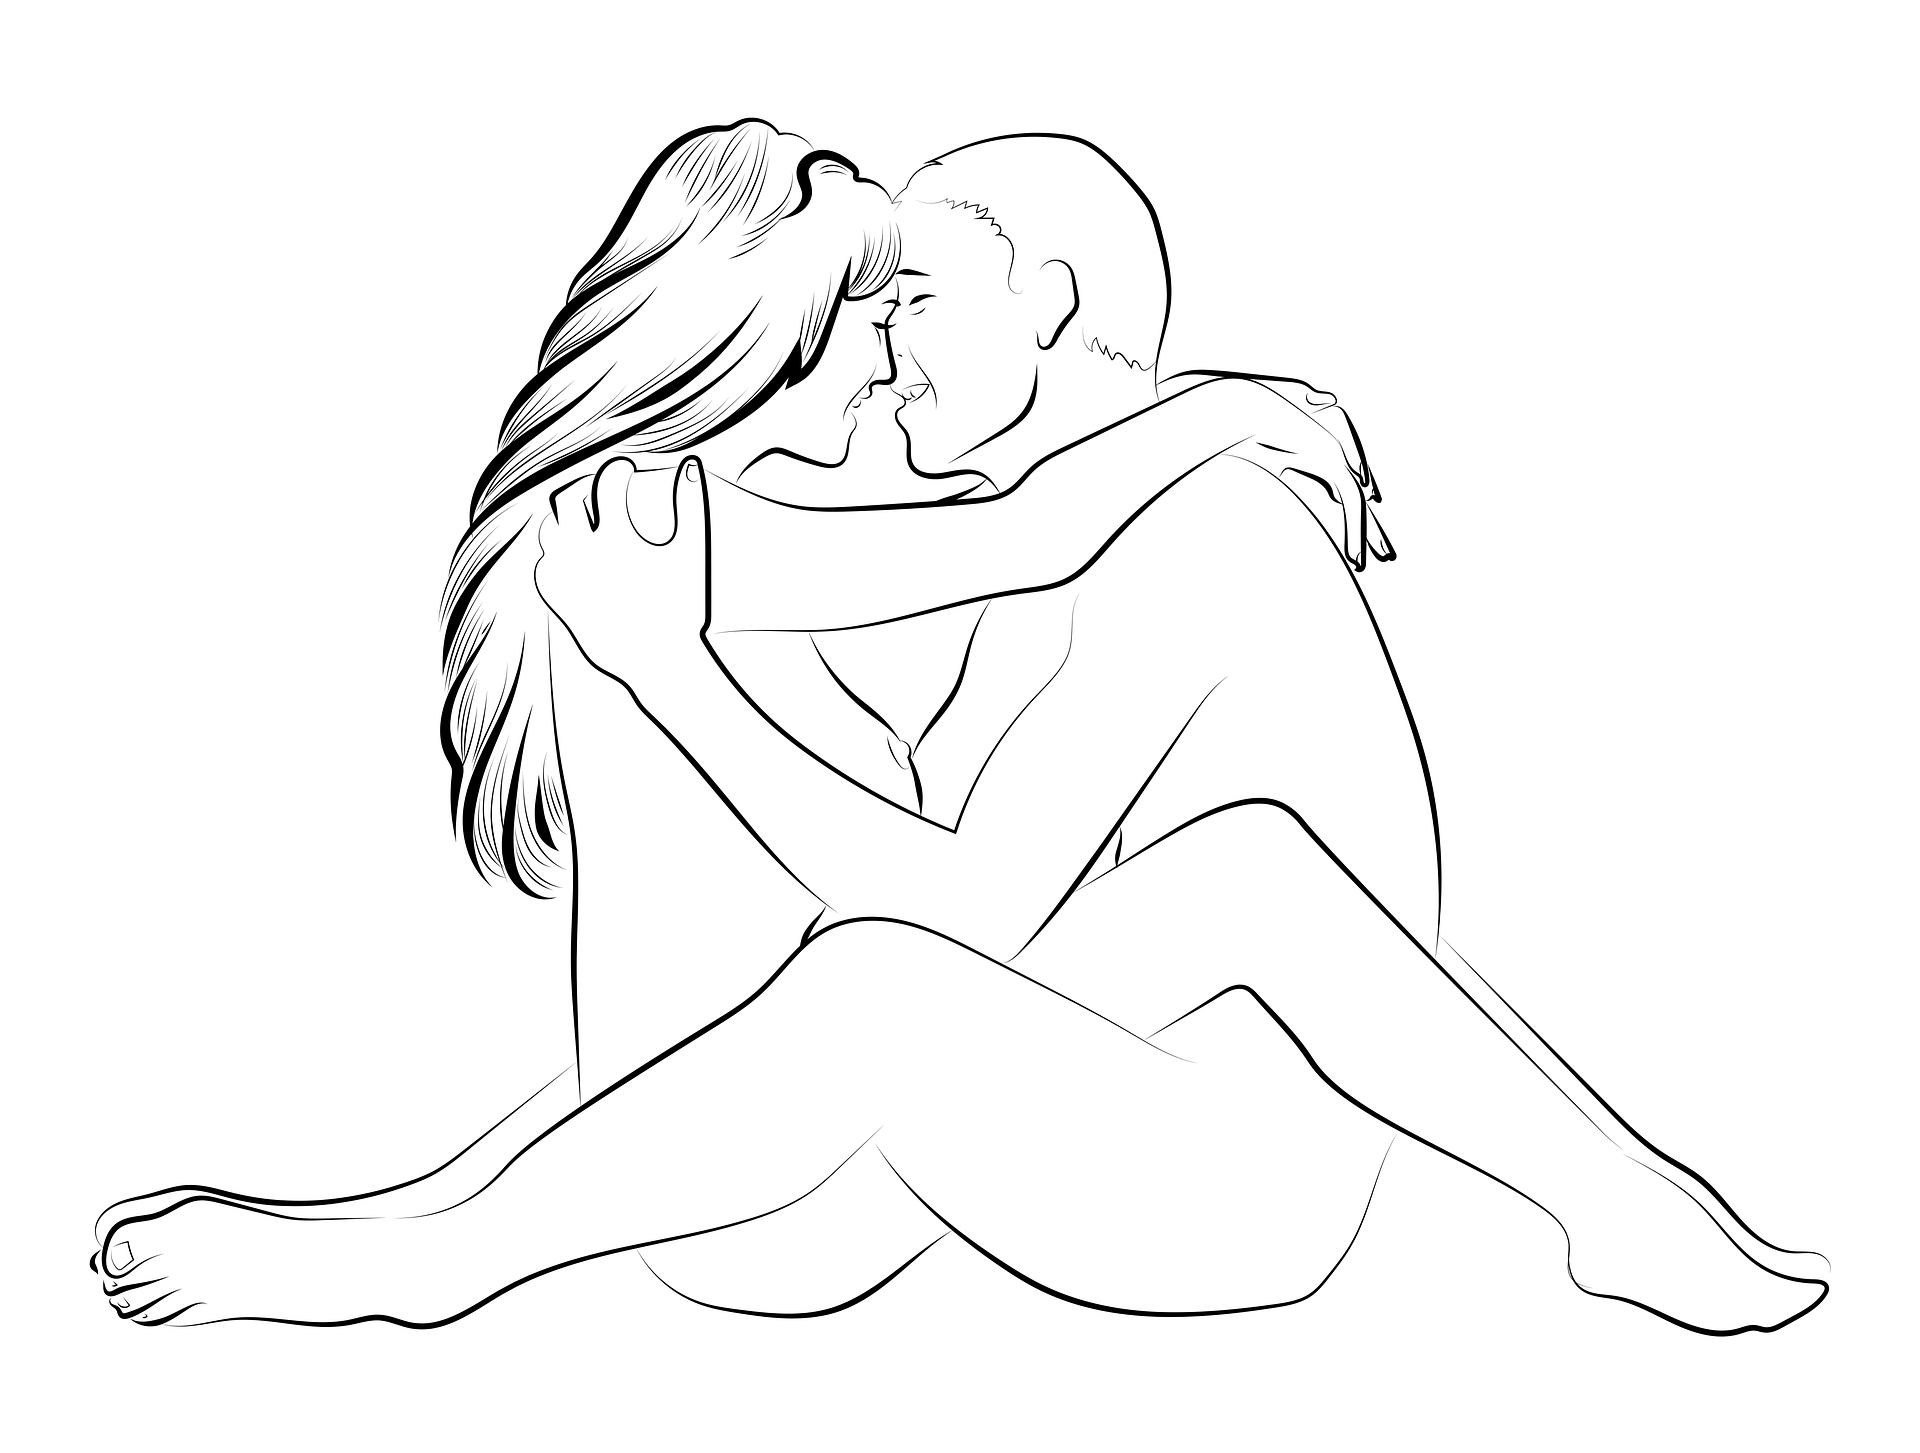
\includegraphics[width=0.7\textwidth]{images/brev72.png}
\end{center}

\breakpage
